\section{Namespace: Global}

\begin{figure}[H]
	\centering
	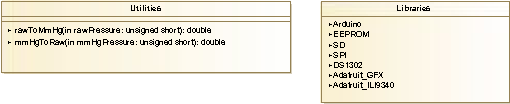
\includegraphics[width=0.6\textwidth]{klassediagram_extra-crop.pdf}
	\caption{Klasse diagram over det globale namespace}\label{fig:classDiagramextra}
\end{figure}

\subsection{Klasse: Utilities}
Denne klasse tilhører det globale namespace og kan tilgås af alle namespaces. Klassen skal ses som en hjælpe klasse med funktion der kan være brugbare flere steder

\subsubsection{Metode: rawToMmHG()}
\textbf{Parameter: } \textit{unsigned short rawPressure}
\\ \textbf{Returtype: } \textit{double}
\\ \textbf{Beskrivelse: } Metoden konverterer rå ADC værdi til mmHg.

\subsubsection{Metode: mmHgToRaw()}
\textbf{Parameter: } \textit{unsigned short mmHgPressure}
\\ \textbf{Returtype: } \textit{double}
\\ \textbf{Beskrivelse: } Metoden konverterer mmHg værdi til rå ACD værdi.

\subsection{Klasse: Konditioneringsapparat.pde (Main fil)}
Denne klasse er softwaren main fil, her samles funktionaliteten i to metoder: \textit{setup()} og l\textit{oop()}, samt 5 interrupt service rutiner. Dette er begge metoder som arduino skal have. \textit{setup()} bliver kørt som først når arduinoen startes og derefter køres det uendeligt \textit{loop()}. Klassen kender kun til de to klasser i GUI laget, Buttons og Display
Da interrupt ikke kan sættes fra andre steder end main filen, bliver der initieret 5 interrupt i denne klasse, hhv to til konditioneringsforløbet, en til okklusionstræning og to til setup.

\subsubsection{Metode: intCon\_ISR(), intBT\_ISR(), intOcc\_ISR(), intCha\_ISR() og intSel\_ISR()}
\textbf{Parameter: } \textit{void}
\\ \textbf{Returtype: } \textit{void}
\\ \textbf{Beskrivelse: } Disse fem interrupt service rutiner kalder alle sammen deres respektive metode fra klassen Buttons. Alle metoder indeholder et delay på 100 ms og derefter et if statement, som tjekker om interrupt pin’en stadig er høj, dette software imødekommer debouncing, se afsnit \ref{title:buttons}


\subsubsection{Metode: setup()}
\textbf{Parameter: } \textit{void}
\\ \textbf{Returtype: } \textit{void}
\\ \textbf{Beskrivelse: } Denne metode bruges til opsætning af arduino, og det er derfor også her at det afgøres om arduinoen skal køre hhv konditioneringsforløb, okklusionstræning eller setup. Derfor aflæses værdien af 3 digital porte for at afgøre hvilket program der skal køres. Derefter opsættes de respektive interrupt for det valgt program. Dette er nødvendigt da prototypen kun har 2 knapper og disse skifter funktion efter hvilket program der er valgt
\begin{lstlisting}
	programToRun = btt.readModeSwitch();
	
	//Setup for i interrupts
	pinMode(interruptPin0, INPUT);
	pinMode(interruptPin1, INPUT);
	
	switch(btt.readModeSwitch()){
	case 1: //Conditioning
	attachInterrupt(digitalPinToInterrupt(interruptPin0), intCon_ISR, RISING);
	attachInterrupt(digitalPinToInterrupt(interruptPin1), intBT_ISR, RISING);
	break;
	case 2: //Occlusion
	attachInterrupt(digitalPinToInterrupt(interruptPin0), intOcc_ISR, RISING);
	break;
	case 3: //Setup
	attachInterrupt(digitalPinToInterrupt(interruptPin0), intCha_ISR, RISING);
	attachInterrupt(digitalPinToInterrupt(interruptPin1), intSel_ISR, RISING);
	break;
	}
\end{lstlisting}

\subsubsection{Metode: loop()}
\textbf{Parameter: } \textit{void}
\\ \textbf{Returtype: } \textit{void}
\\ \textbf{Beskrivelse: } Uendeligt loop der eksekveres efter metoden setup() har kørt. Metoden indeholder en switch case struktur, og program valget afgøre hvilken case der køres. Der kan kun skiftes case, hvis arduinoen genstartes. 